\documentclass[tikz, border=1pt]{standalone}
\pdfoutput=1 % if your are submitting a pdflatex (i.e. if you have
             % images in pdf, png or jpg format)

\usepackage{graphicx}

% Use the tikz package
\usepackage{tikz}
\usetikzlibrary{decorations}


\begin{document}

	\begin{tikzpicture}
	
		\node at (0,7.5) {Commutative Case};
	
		\node at (0,6) {

	\begin{tikzpicture}
		
		%horizontal lines
		\draw (0,4)--(6,4);
		\draw (0,4.2)--(6,4.2);
		\draw (0,4.4)--(6,4.4);
		\draw (0,4.6)--(6,4.6);
		\draw (0,4.8)--(6,4.8);
		\draw (0,5)--(6,5);
		\draw (0,5.2)--(6,5.2);
		\draw (0,5.4)--(6,5.4);
		
		%vertical lines
		\draw (3.01,4)--(3.01,5.4);
		\draw (2.99,4)--(2.99,5.4);
		
		%Now draw some 'gates'
		\fill (0.6,4.4) circle[radius=0.08];
		\fill (0.6,5) circle[radius=0.08];
		\draw (0.6,4.4)--(0.6,5);
		
		\fill (1,5) circle[radius=0.08];
		\fill (1,5.4) circle[radius=0.08];
		\draw (1,5)--(1,5.4);
		
		\fill (1.4,4.8) circle[radius=0.08];
		\fill (1.4,4.2) circle[radius=0.08];
		\draw (1.4,4.8)--(1.4,4.2);
		
		\fill (1.8,4.2) circle[radius=0.08];
		\fill (1.8,4.4) circle[radius=0.08];
		\draw (1.8,4.2)--(1.8,4.4);
		
		\fill (2.2,5.2) circle[radius=0.08];
		\fill (2.2,4.4) circle[radius=0.08];
		\draw (2.2,4.4)--(2.2,5.2);
		
		\fill (2.6,5) circle[radius=0.08];
		\fill (2.6,4.4) circle[radius=0.08];
		\draw (2.6,5)--(2.6,4.4);
		
		%halfway mark
		
		\fill (3.4,5) circle[radius=0.08];
		\fill (3.4,4.4) circle[radius=0.08];
		\draw (3.4,5)--(3.4,4.4);
		
		\fill (3.8,4.8) circle[radius=0.08];
		\fill (3.8,5.2) circle[radius=0.08];
		\draw (3.8,4.8)--(3.8,5.2);
		
		\fill (4.2,4) circle[radius=0.08];
		\fill (4.2,5.2) circle[radius=0.08];
		\draw (4.2,4)--(4.2,5.2);
		
		\fill (4.6,4.2) circle[radius=0.08];
		\fill (4.6,4.8) circle[radius=0.08];
		\draw (4.6,4.2)--(4.6,4.8);
		
		\fill (5,5.4) circle[radius=0.08];
		\fill (5,5) circle[radius=0.08];
		\draw (5,5.4)--(5,5);
		
		\fill (5.4,4.4) circle[radius=0.08];
		\fill (5.4,5) circle[radius=0.08];
		\draw (5.4,4.4)--(5.4,5);
		
	\end{tikzpicture}
		
		};
		
		\node at (0,4) {

	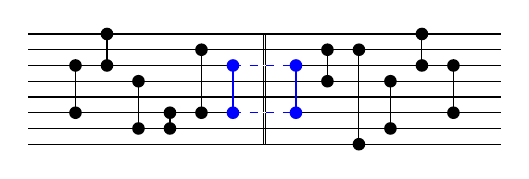
\begin{tikzpicture}
		
		%horizontal lines
		\draw (0,4)--(6,4);
		\draw (0,4.2)--(6,4.2);
		\draw (0,4.4)--(6,4.4);
		\draw (0,4.6)--(6,4.6);
		\draw (0,4.8)--(6,4.8);
		\draw (0,5)--(6,5);
		\draw (0,5.2)--(6,5.2);
		\draw (0,5.4)--(6,5.4);
		
		%vertical lines
		\draw (3.01,4)--(3.01,5.4);
		\draw (2.99,4)--(2.99,5.4);
		
		%Now draw some 'gates'
		\fill (0.6,4.4) circle[radius=0.08];
		\fill (0.6,5) circle[radius=0.08];
		\draw (0.6,4.4)--(0.6,5);
		
		\fill (1,5) circle[radius=0.08];
		\fill (1,5.4) circle[radius=0.08];
		\draw (1,5)--(1,5.4);
		
		\fill (1.4,4.8) circle[radius=0.08];
		\fill (1.4,4.2) circle[radius=0.08];
		\draw (1.4,4.8)--(1.4,4.2);
		
		\fill (1.8,4.2) circle[radius=0.08];
		\fill (1.8,4.4) circle[radius=0.08];
		\draw (1.8,4.2)--(1.8,4.4);
		
		\fill (2.2,5.2) circle[radius=0.08];
		\fill (2.2,4.4) circle[radius=0.08];
		\draw (2.2,4.4)--(2.2,5.2);
		
		\fill[blue] (2.6,5) circle[radius=0.08];
		\fill[blue] (2.6,4.4) circle[radius=0.08];
		\draw[blue] (2.6,5)--(2.6,4.4);
		
		\draw[white] (2.6,5)--(3.4,5);
		\draw[blue,dashed] (2.6,5)--(3.4,5);
		
		\draw[white] (2.6,4.4)--(3.4,4.4);
		\draw[blue,dashed] (2.6,4.4)--(3.4,4.4);
		
		%halfway mark
		
		\fill[blue] (3.4,5) circle[radius=0.08];
		\fill[blue] (3.4,4.4) circle[radius=0.08];
		\draw[blue] (3.4,5)--(3.4,4.4);
		
		\fill (3.8,4.8) circle[radius=0.08];
		\fill (3.8,5.2) circle[radius=0.08];
		\draw (3.8,4.8)--(3.8,5.2);
		
		\fill (4.2,4) circle[radius=0.08];
		\fill (4.2,5.2) circle[radius=0.08];
		\draw (4.2,4)--(4.2,5.2);
		
		\fill (4.6,4.2) circle[radius=0.08];
		\fill (4.6,4.8) circle[radius=0.08];
		\draw (4.6,4.2)--(4.6,4.8);
		
		\fill (5,5.4) circle[radius=0.08];
		\fill (5,5) circle[radius=0.08];
		\draw (5,5.4)--(5,5);
		
		\fill (5.4,4.4) circle[radius=0.08];
		\fill (5.4,5) circle[radius=0.08];
		\draw (5.4,4.4)--(5.4,5);
		
	\end{tikzpicture}
		};
		
		\node at (0,2) {

	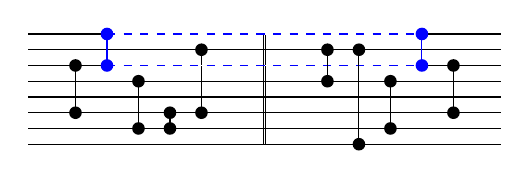
\begin{tikzpicture}
		
		%horizontal lines
		\draw (0,4)--(6,4);
		\draw (0,4.2)--(6,4.2);
		\draw (0,4.4)--(6,4.4);
		\draw (0,4.6)--(6,4.6);
		\draw (0,4.8)--(6,4.8);
		\draw (0,5)--(6,5);
		\draw (0,5.2)--(6,5.2);
		\draw (0,5.4)--(6,5.4);
		
		%vertical lines
		\draw (3.01,4)--(3.01,5.4);
		\draw (2.99,4)--(2.99,5.4);
		
		%Now draw some 'gates'
		\fill (0.6,4.4) circle[radius=0.08];
		\fill (0.6,5) circle[radius=0.08];
		\draw (0.6,4.4)--(0.6,5);
		
		\fill[blue] (1,5) circle[radius=0.08];
		\fill[blue] (1,5.4) circle[radius=0.08];
		\draw[blue] (1,5)--(1,5.4);
		
		\fill (1.4,4.8) circle[radius=0.08];
		\fill (1.4,4.2) circle[radius=0.08];
		\draw (1.4,4.8)--(1.4,4.2);
		
		\fill (1.8,4.2) circle[radius=0.08];
		\fill (1.8,4.4) circle[radius=0.08];
		\draw (1.8,4.2)--(1.8,4.4);
		
		\fill (2.2,5.2) circle[radius=0.08];
		\fill (2.2,4.4) circle[radius=0.08];
		\draw (2.2,4.4)--(2.2,5.2);
		
		\draw[white] (1,5)--(5,5);
		\draw[blue,dashed] (1,5)--(5,5);
		
		\draw[white] (1,5.4)--(5,5.4);
		\draw[blue,dashed] (1,5.4)--(5,5.4);	
		
		%halfway mark
		
		\fill (3.8,4.8) circle[radius=0.08];
		\fill (3.8,5.2) circle[radius=0.08];
		\draw (3.8,4.8)--(3.8,5.2);
		
		\fill (4.2,4) circle[radius=0.08];
		\fill (4.2,5.2) circle[radius=0.08];
		\draw (4.2,4)--(4.2,5.2);
		
		\fill (4.6,4.2) circle[radius=0.08];
		\fill (4.6,4.8) circle[radius=0.08];
		\draw (4.6,4.2)--(4.6,4.8);
		
		\fill[blue] (5,5.4) circle[radius=0.08];
		\fill[blue] (5,5) circle[radius=0.08];
		\draw[blue] (5,5.4)--(5,5);
		
		\fill (5.4,4.4) circle[radius=0.08];
		\fill (5.4,5) circle[radius=0.08];
		\draw (5.4,4.4)--(5.4,5);
		
	\end{tikzpicture}
		
		};
		
		\node at (0,0) {

	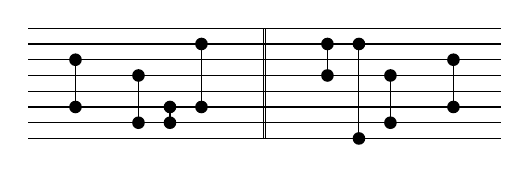
\begin{tikzpicture}
		
		%horizontal lines
		\draw (0,4)--(6,4);
		\draw (0,4.2)--(6,4.2);
		\draw (0,4.4)--(6,4.4);
		\draw (0,4.6)--(6,4.6);
		\draw (0,4.8)--(6,4.8);
		\draw (0,5)--(6,5);
		\draw (0,5.2)--(6,5.2);
		\draw (0,5.4)--(6,5.4);
		
		%vertical lines
		\draw (3.01,4)--(3.01,5.4);
		\draw (2.99,4)--(2.99,5.4);
		
		%Now draw some 'gates'
		\fill (0.6,4.4) circle[radius=0.08];
		\fill (0.6,5) circle[radius=0.08];
		\draw (0.6,4.4)--(0.6,5);
		
		\fill (1.4,4.8) circle[radius=0.08];
		\fill (1.4,4.2) circle[radius=0.08];
		\draw (1.4,4.8)--(1.4,4.2);
		
		\fill (1.8,4.2) circle[radius=0.08];
		\fill (1.8,4.4) circle[radius=0.08];
		\draw (1.8,4.2)--(1.8,4.4);
		
		\fill (2.2,5.2) circle[radius=0.08];
		\fill (2.2,4.4) circle[radius=0.08];
		\draw (2.2,4.4)--(2.2,5.2);	
		
		%halfway mark
		
		\fill (3.8,4.8) circle[radius=0.08];
		\fill (3.8,5.2) circle[radius=0.08];
		\draw (3.8,4.8)--(3.8,5.2);
		
		\fill (4.2,4) circle[radius=0.08];
		\fill (4.2,5.2) circle[radius=0.08];
		\draw (4.2,4)--(4.2,5.2);
		
		\fill (4.6,4.2) circle[radius=0.08];
		\fill (4.6,4.8) circle[radius=0.08];
		\draw (4.6,4.2)--(4.6,4.8);
		
		\fill (5.4,4.4) circle[radius=0.08];
		\fill (5.4,5) circle[radius=0.08];
		\draw (5.4,4.4)--(5.4,5);
		
	\end{tikzpicture}
		
		};
	
		\node at (7,7.5) {Non-Commutative Case};
	
		\node at (7,6) {

	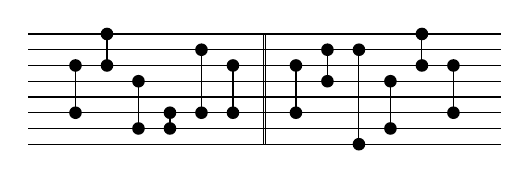
\begin{tikzpicture}
		
		%horizontal lines
		\draw (0,4)--(6,4);
		\draw (0,4.2)--(6,4.2);
		\draw (0,4.4)--(6,4.4);
		\draw (0,4.6)--(6,4.6);
		\draw (0,4.8)--(6,4.8);
		\draw (0,5)--(6,5);
		\draw (0,5.2)--(6,5.2);
		\draw (0,5.4)--(6,5.4);
		
		%vertical lines
		\draw (3.01,4)--(3.01,5.4);
		\draw (2.99,4)--(2.99,5.4);
		
		%Now draw some 'gates'
		\fill (0.6,4.4) circle[radius=0.08];
		\fill (0.6,5) circle[radius=0.08];
		\draw (0.6,4.4)--(0.6,5);
		
		\fill (1,5) circle[radius=0.08];
		\fill (1,5.4) circle[radius=0.08];
		\draw (1,5)--(1,5.4);
		
		\fill (1.4,4.8) circle[radius=0.08];
		\fill (1.4,4.2) circle[radius=0.08];
		\draw (1.4,4.8)--(1.4,4.2);
		
		\fill (1.8,4.2) circle[radius=0.08];
		\fill (1.8,4.4) circle[radius=0.08];
		\draw (1.8,4.2)--(1.8,4.4);
		
		\fill (2.2,5.2) circle[radius=0.08];
		\fill (2.2,4.4) circle[radius=0.08];
		\draw (2.2,4.4)--(2.2,5.2);
		
		\fill (2.6,5) circle[radius=0.08];
		\fill (2.6,4.4) circle[radius=0.08];
		\draw (2.6,5)--(2.6,4.4);
		
		%halfway mark
		
		\fill (3.4,5) circle[radius=0.08];
		\fill (3.4,4.4) circle[radius=0.08];
		\draw (3.4,5)--(3.4,4.4);
		
		\fill (3.8,4.8) circle[radius=0.08];
		\fill (3.8,5.2) circle[radius=0.08];
		\draw (3.8,4.8)--(3.8,5.2);
		
		\fill (4.2,4) circle[radius=0.08];
		\fill (4.2,5.2) circle[radius=0.08];
		\draw (4.2,4)--(4.2,5.2);
		
		\fill (4.6,4.2) circle[radius=0.08];
		\fill (4.6,4.8) circle[radius=0.08];
		\draw (4.6,4.2)--(4.6,4.8);
		
		\fill (5,5.4) circle[radius=0.08];
		\fill (5,5) circle[radius=0.08];
		\draw (5,5.4)--(5,5);
		
		\fill (5.4,4.4) circle[radius=0.08];
		\fill (5.4,5) circle[radius=0.08];
		\draw (5.4,4.4)--(5.4,5);
		
	\end{tikzpicture}
		
		};
		
		\node at (7,4) {

	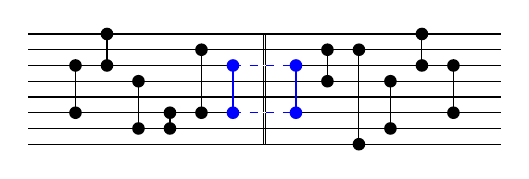
\begin{tikzpicture}
		
		%horizontal lines
		\draw (0,4)--(6,4);
		\draw (0,4.2)--(6,4.2);
		\draw (0,4.4)--(6,4.4);
		\draw (0,4.6)--(6,4.6);
		\draw (0,4.8)--(6,4.8);
		\draw (0,5)--(6,5);
		\draw (0,5.2)--(6,5.2);
		\draw (0,5.4)--(6,5.4);
		
		%vertical lines
		\draw (3.01,4)--(3.01,5.4);
		\draw (2.99,4)--(2.99,5.4);
		
		%Now draw some 'gates'
		\fill (0.6,4.4) circle[radius=0.08];
		\fill (0.6,5) circle[radius=0.08];
		\draw (0.6,4.4)--(0.6,5);
		
		\fill (1,5) circle[radius=0.08];
		\fill (1,5.4) circle[radius=0.08];
		\draw (1,5)--(1,5.4);
		
		\fill (1.4,4.8) circle[radius=0.08];
		\fill (1.4,4.2) circle[radius=0.08];
		\draw (1.4,4.8)--(1.4,4.2);
		
		\fill (1.8,4.2) circle[radius=0.08];
		\fill (1.8,4.4) circle[radius=0.08];
		\draw (1.8,4.2)--(1.8,4.4);
		
		\fill (2.2,5.2) circle[radius=0.08];
		\fill (2.2,4.4) circle[radius=0.08];
		\draw (2.2,4.4)--(2.2,5.2);
		
		\fill[blue] (2.6,5) circle[radius=0.08];
		\fill[blue] (2.6,4.4) circle[radius=0.08];
		\draw[blue] (2.6,5)--(2.6,4.4);
		
		\draw[white] (2.6,5)--(3.4,5);
		\draw[blue,dashed] (2.6,5)--(3.4,5);
		
		\draw[white] (2.6,4.4)--(3.4,4.4);
		\draw[blue,dashed] (2.6,4.4)--(3.4,4.4);	
		
		%halfway mark
		
		\fill[blue] (3.4,5) circle[radius=0.08];
		\fill[blue] (3.4,4.4) circle[radius=0.08];
		\draw[blue] (3.4,5)--(3.4,4.4);
		
		\fill (3.8,4.8) circle[radius=0.08];
		\fill (3.8,5.2) circle[radius=0.08];
		\draw (3.8,4.8)--(3.8,5.2);
		
		\fill (4.2,4) circle[radius=0.08];
		\fill (4.2,5.2) circle[radius=0.08];
		\draw (4.2,4)--(4.2,5.2);
		
		\fill (4.6,4.2) circle[radius=0.08];
		\fill (4.6,4.8) circle[radius=0.08];
		\draw (4.6,4.2)--(4.6,4.8);
		
		\fill (5,5.4) circle[radius=0.08];
		\fill (5,5) circle[radius=0.08];
		\draw (5,5.4)--(5,5);
		
		\fill (5.4,4.4) circle[radius=0.08];
		\fill (5.4,5) circle[radius=0.08];
		\draw (5.4,4.4)--(5.4,5);
		
	\end{tikzpicture}
		};
		
		\node at (7,2) {

	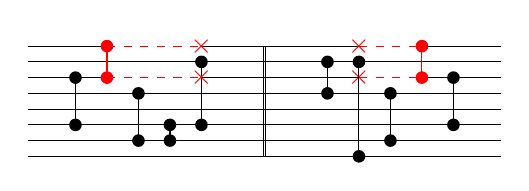
\begin{tikzpicture}
		
		%horizontal lines
		\draw (0,4)--(6,4);
		\draw (0,4.2)--(6,4.2);
		\draw (0,4.4)--(6,4.4);
		\draw (0,4.6)--(6,4.6);
		\draw (0,4.8)--(6,4.8);
		\draw (0,5)--(6,5);
		\draw (0,5.2)--(6,5.2);
		\draw (0,5.4)--(6,5.4);
		
		%vertical lines
		\draw (3.01,4)--(3.01,5.4);
		\draw (2.99,4)--(2.99,5.4);
		
		%Now draw some 'gates'
		\fill (0.6,4.4) circle[radius=0.08];
		\fill (0.6,5) circle[radius=0.08];
		\draw (0.6,4.4)--(0.6,5);
		
		\fill[red] (1,5) circle[radius=0.08];
		\fill[red] (1,5.4) circle[radius=0.08];
		\draw[red] (1,5)--(1,5.4);
		
		\fill (1.4,4.8) circle[radius=0.08];
		\fill (1.4,4.2) circle[radius=0.08];
		\draw (1.4,4.8)--(1.4,4.2);
		
		\fill (1.8,4.2) circle[radius=0.08];
		\fill (1.8,4.4) circle[radius=0.08];
		\draw (1.8,4.2)--(1.8,4.4);
		
		\fill (2.2,5.2) circle[radius=0.08];
		\fill (2.2,4.4) circle[radius=0.08];
		\draw (2.2,4.4)--(2.2,5.2);
		
		\draw[white] (1,5)--(2.2,5);
		\draw[red,dashed] (1,5)--(2.2,5);
		
		\draw[white] (4.2,5)--(5,5);
		\draw[red,dashed] (4.2,5)--(5,5);
		
		\draw[white] (1,5.4)--(2.2,5.4);
		\draw[red,dashed] (1,5.4)--(2.2,5.4);
		
		\draw[white] (4.2,5.4)--(5,5.4);
		\draw[red,dashed] (4.2,5.4)--(5,5.4);
		
		\node[red] at (2.2,5) {$\times$};	
		\node[red] at (4.2,5) {$\times$};	
		\node[red] at (2.2,5.4) {$\times$};	
		\node[red] at (4.2,5.4) {$\times$};
		
		%halfway mark
		
		\fill (3.8,4.8) circle[radius=0.08];
		\fill (3.8,5.2) circle[radius=0.08];
		\draw (3.8,4.8)--(3.8,5.2);
		
		\fill (4.2,4) circle[radius=0.08];
		\fill (4.2,5.2) circle[radius=0.08];
		\draw (4.2,4)--(4.2,5.2);
		
		\fill (4.6,4.2) circle[radius=0.08];
		\fill (4.6,4.8) circle[radius=0.08];
		\draw (4.6,4.2)--(4.6,4.8);
		
		\fill[red] (5,5.4) circle[radius=0.08];
		\fill[red] (5,5) circle[radius=0.08];
		\draw[red] (5,5.4)--(5,5);
		
		\fill (5.4,4.4) circle[radius=0.08];
		\fill (5.4,5) circle[radius=0.08];
		\draw (5.4,4.4)--(5.4,5);
		
	\end{tikzpicture}
		
		};
		
		\node at (7,0) {

	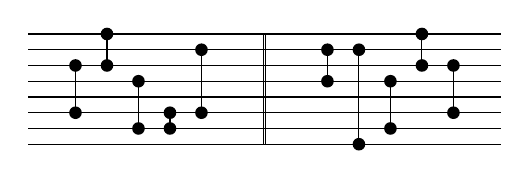
\begin{tikzpicture}
		
		%horizontal lines
		\draw (0,4)--(6,4);
		\draw (0,4.2)--(6,4.2);
		\draw (0,4.4)--(6,4.4);
		\draw (0,4.6)--(6,4.6);
		\draw (0,4.8)--(6,4.8);
		\draw (0,5)--(6,5);
		\draw (0,5.2)--(6,5.2);
		\draw (0,5.4)--(6,5.4);
		
		%vertical lines
		\draw (3.01,4)--(3.01,5.4);
		\draw (2.99,4)--(2.99,5.4);
		
		%Now draw some 'gates'
		\fill (0.6,4.4) circle[radius=0.08];
		\fill (0.6,5) circle[radius=0.08];
		\draw (0.6,4.4)--(0.6,5);
		
		\fill (1,5) circle[radius=0.08];
		\fill (1,5.4) circle[radius=0.08];
		\draw (1,5)--(1,5.4);
		
		\fill (1.4,4.8) circle[radius=0.08];
		\fill (1.4,4.2) circle[radius=0.08];
		\draw (1.4,4.8)--(1.4,4.2);
		
		\fill (1.8,4.2) circle[radius=0.08];
		\fill (1.8,4.4) circle[radius=0.08];
		\draw (1.8,4.2)--(1.8,4.4);
		
		\fill (2.2,5.2) circle[radius=0.08];
		\fill (2.2,4.4) circle[radius=0.08];
		\draw (2.2,4.4)--(2.2,5.2);	
		
		%halfway mark
		
		\fill (3.8,4.8) circle[radius=0.08];
		\fill (3.8,5.2) circle[radius=0.08];
		\draw (3.8,4.8)--(3.8,5.2);
		
		\fill (4.2,4) circle[radius=0.08];
		\fill (4.2,5.2) circle[radius=0.08];
		\draw (4.2,4)--(4.2,5.2);
		
		\fill (4.6,4.2) circle[radius=0.08];
		\fill (4.6,4.8) circle[radius=0.08];
		\draw (4.6,4.2)--(4.6,4.8);
		
		\fill (5,5.4) circle[radius=0.08];
		\fill (5,5) circle[radius=0.08];
		\draw (5,5.4)--(5,5);
		
		\fill (5.4,4.4) circle[radius=0.08];
		\fill (5.4,5) circle[radius=0.08];
		\draw (5.4,4.4)--(5.4,5);
		
	\end{tikzpicture}
		};
		
	\end{tikzpicture}

\end{document}
